%\documentclass[aspectratio=169]{beamer}
\documentclass{beamer}
\usetheme{PaloAlto}
%\usetheme{AnnArbor}

\usepackage[utf8]{inputenc}

\title{Curso de BEAMER.}
\author[Felipe]{Felipe F. Soares.}
\institute[UFC]{Universidade Federal do Ceará \\ ufc.br}
\date{2016}
%\date{}
%\date{Nome do evento, 2016}
\logo{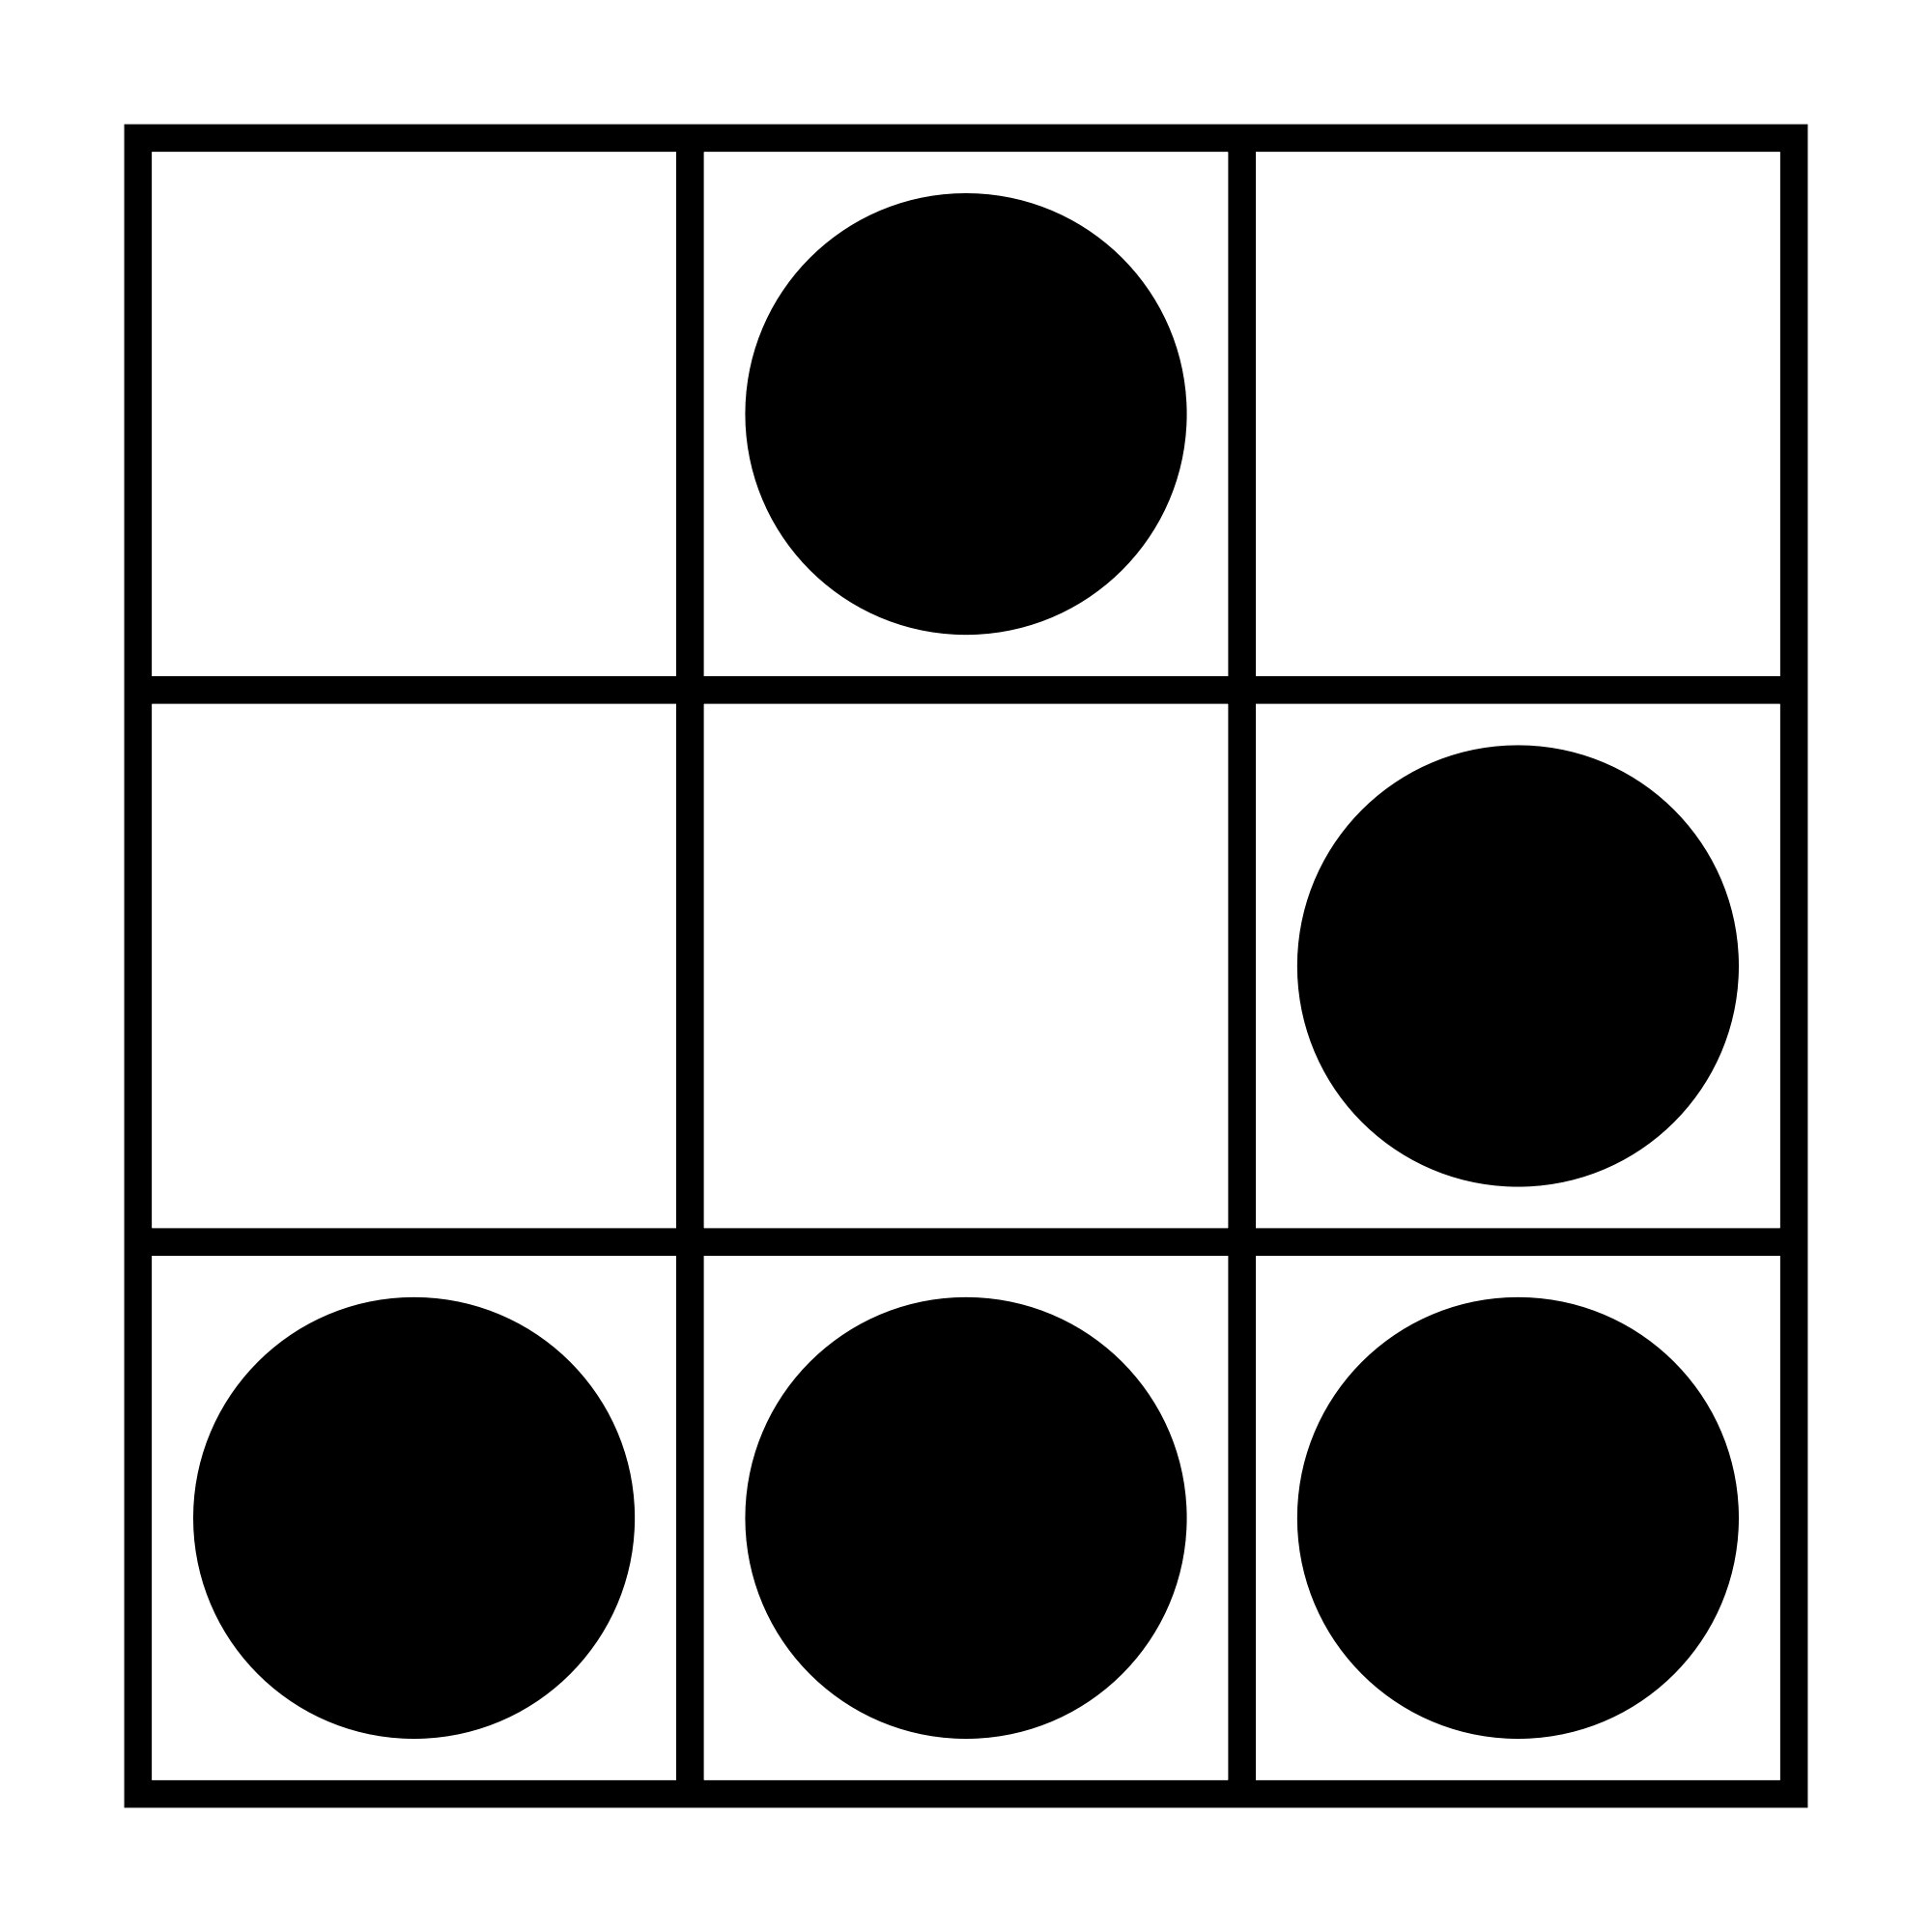
\includegraphics[scale=0.01]{images/glider.png}}

\begin{document}
	\begin{frame}{Esse é o título do quadro}
		\titlepage
	\end{frame}
	
	\begin{frame}
		\frametitle{Esse é o título do quadro}
		\framesubtitle{Esse é o subtítulo}
		Aqui vem o texto do quadro!
		
		\alert{Esse ficará em destaque.} \pause
		\begin{block}{Aqui vem o título do bloco}
			Aqui vem um texto
		\end{block} \pause
		
		\begin{block}
			Aqui vem o texto do outro bloco
		\end{block} \pause
		
		\begin{block}{}
			Aqui vem o texto do outro bloco
		\end{block} \pause
		
		\begin{block}{\ }
			Aqui vem o texto do outro bloco
		\end{block}
	\end{frame}
\end{document}